\chapter{Mentale Modelle} % (fold)
\label{cha:mentale_modelle}

In diesem Kapitel wird das Konzept der mentalen Modelle eingeführt, das in dieser Arbeit als Erklärungsansatz für jene Aspekte von "Articulation Work" verwendet wird, die die nicht sichtbaren, kognitiven Beiträge eines beteiligten Individuums betreffen. Nach einer Einführung in die Begriffswelt der mentalen Modelle wird die Argumentation aus dem letzten Kapitel nochmals aufgegriffen und die mögliche Rolle mentaler Modelle für "Articulation Work" erörtert. In der Folge werden Methoden eingeführt mit denen mentale Modelle externalisiert und kommuniziert werden können. Basierend auf diesen Beschreibungen wird im letzten Teil des Kapitels untersucht, welche Herausforderungen sich bei der Anwendung dieser Methoden im Kontext von "Articulation Work" ergeben können.

\section{Articulation Work und mentale Modelle} % (fold)
\label{sec:articulation_work_und_mentale_modelle}

Wie bereits im vorgehenden Kapitel beschrieben, wird in vorhandenen Arbeiten zu Articulation Work deren Auftreten, Kontext und Wirkung beschrieben, nicht aber die individuellen Aspekte ihrer Durchführung. Der eigentliche Gegenstand der Abstimmung, die im Rahmen der Articulation Work erfolgen soll, wird ebenfalls nicht konkret festgelegt. Strauss spricht von \emph{„putting together tasks, task sequences, task clusters - even aligning larger units such as lines of work and subprojects - in the service of work flow“} \citep[][S. 2]{Strauss88}, und konkretisiert \emph{„the specific questions about tasks of course include: what, where, when, how, for how long, how complex, how weIl defined are their boundaries, how attainable are they under current working conditions, how precisely are they defined in their operational details, and what is the expected level of performance. (Which of those are the most salient dimensions depends on the organizational work context under study, and we cannot emphasize too much that \textbf{it is the researcher who must discover these saliences}.)“} \citep[][S. 6]{Strauss85}. Strauss lässt also offen, was es exakt ist, dass abgestimmt werden muss bzw. verlagert diese Frage in den konkreten Einzelfall. 

Strauss spricht diese Auslassung in einer späteren Arbeit explizit an \citep[][S. 131]{Strauss93} und beschäftigt sich in dieser auch mit jenen kognitiven Vorgängen, die von ihm als „thought processes“ oder „mental activities“ bezeichnet werden und die untrennbar mit jeder Art von Tätigkeit und Interaktion verbunden sind \citep[][S. 146]{Strauss93} und diese beeinflussen \citep[][S. 132]{Strauss93}.  

Im Kontext der Abstimmung von Tätigkeiten kommt den „thought processes“ der Individuen große Bedeutung zu, da sie den sichtbaren individuellen Handlungen zugrunde liegen bzw. diese beeinflussen. „Articulation Work“ wirkt sich also auf die „thought processes“ der beteiligten Individuen aus. „Thought processes“ umfassen \emph{„images, imaginations, projections of scenes, [...] flashes of insight, rehearsals of action, construction and reconstruction of scenarios,  the spurting up of metaphors or comparisons, the reworking and reevaluating of past scenes and one's actions within them, and so on and on“} \citep[][S. 130]{Strauss93} - also im Wesentlichen alle kognitiven Vorgänge, die unmittelbar oder mittelbar im Zusammenhang mit den sichtbaren Arbeitsaspekten, insbesondere den Tätigkeiten zur Zielerreichung und der wahrgenommenen Arbeitsumgebung, stehen. Strauss interessiert sich allerdings ausschließlich für die dynamischen Aspekte der Interaktion zwischen Individuen, nicht aber für die Ausgangspunkte und Ergebnisse der zugrunde liegenden „thought processes“ \citep[][S. 149]{Strauss93}

% section articulation_work_und_mentale_modelle (end)

\section{Begriffsbestimmung} % (fold)
\label{sec:begriffsbestimmung}

% section begriffsbestimmung (end)

Das Konzept der "mentalen Modelle" wird grundsätzlich verwendet, um zu erklären \emph{„wie Menschen die Welt verstehen -- genauer: wie sie ihr Wissen benutzen, um sich bestimmte Phänomene der Welt subjektiv plausibel zu machen“} \citep[][S. VII]{Seel91}. Mentale Modelle sind dabei Erklärungsmodelle der Welt, die Menschen auf Basis von Alltagserfahrungen, bisherigem Wissen und darauf basierenden Schlussfolgerungen bilden. Ein gebildetes mentales Modell wird dann als Basis verwendet, um die Welt zu verstehen und ggf. Vorhersagen über deren Verhalten zu bilden. \citep[][S. VII]{Seel91}

Im Wesentlichen wurde das Forschungsfeld der mentalen Modelle durch zwei Arbeiten maßgeblich beeinflusst. \citet{Johnson-Laird81} und \citet{Kleer81} führen den Begriff als eigenständigen Forschungsgegenstand ein und legen damit die Grundlage für einen Großteil der nachfolgenden Arbeiten in dem Gebiet. Im Kontext dieser Arbeit werden dabei zwei dieser nachfolgenden Arbeiten näher betrachtet. Zum einen stellt \citet{Norman83} den Begriff erstmals im den Kontext der Mensch-Maschine-Interaktion dar. Zum anderen versucht \citet{Seel91} die unterschiedlichen Richtungen der Forschung im Bereich der mentalen Modelle zusammenzuführen und daraus die Bedeutung von Mentalen Modellen für Lernvorgänge (unter die -- im breiten Verständnis von Seel -- auch die hier relevanten Abstimmungsvorgänge fallen) und Möglichkeiten zu deren Unterstützung abzuleiten. Die folgenden Ausführungen basieren deshalb auf den Ausführungen von \citeauthor{Seel91} und seiner Mitarbeiter (\citet{Ifenthaler06}, \citet{Pirnay-Dummer06} und \citet{Hanke06}).

Mentale Modelle sind nach \citet[][S. 7]{Ifenthaler06} \emph{„kognitive Konstruktionen, die abhängig von der jeweiligen Situation und vom semantischen Wissen einer Persone ad hoc konstruiert werden“}. Ein mentales Modell ist also kein permanentes kognitives Konstrukt, sondern wird auf Basis vorhandenen Wissens in bestimmten Situationen ad-hoc gebildet (siehe dazu auch Abschnitt \ref{sec:bildung_mentaler_modelle}). In engem Zusammenhang mit dem Begriff der mentalen Modelle ist jener der „Schemata“ bei zu nennen. „Schemata“ unterscheiden sich ihrer Definition nach nur in Detail von „mentalen Modellen“\footnote{Tatsächlich wird nach \citet{Ifenthaler06} der Begriff der „mentalen Modelle“ von manchen Autoren zugunsten von „Schemata“ als überflüssig bezeichnet, da zweitere die auftretenden kognitiven Phänomene ausreichend beschreiben würden.} Ein „Schema“ repräsentiert nach \citet[][S. 57]{Seel03a} \emph{„das aufgrund vielfältiger Einzelerfahrungen mit Objekten, Personen, Situationen und Handlungen erworbene verallgemeinerbare und abstrakte Wissen einer Person.“} Schemata werden benutzt um \emph{„Wissensstrukturen zu beschreiben, welche typische Zusammenhänge eines Realitätsbereiches repräsentieren.“} \citep[][S. 8]{Ifenthaler06}. Auf Basis dieser „Schemata“ treffen Individuen treffen Handlungsentscheidungen in bestimmten Situationen. „Schemata“ sind dabei als „Vorlagen“ zu sehen, die adäquate Handlungen für einen bestimmten Situationstypus vorgeben (im Sinne der erwähnten „Verallgemeinerbarkeit“) und Individuen damit zur raschen, unmittelbaren Handlung befähigt, ohne ausführliche Planungstätigkeiten durchführen zu müssen. In Abgrenzung dazu werden „mentale Modelle“ ad-hoc in Situationen gebildet, wo keine Schemata vorhanden sind oder vorhandene nicht angewandt werden können. 

\citet{Ifenthaler06} beschreibt den Zusammenhang zwischen Schemata und mentalen Modellen wie in Abbildung \ref{fig:img_MentaleModelle_iffenthaler_assimilation_akkommodation} dargestellt. Er bezieht sich dabei auf das „Äquilibrations“-Prinzip nach \citet{Piaget76}. Demnach entwickelt sich das Wissen eines Indiviuums durch die komplementären Prozesse „Assimilation“ und „Akkommodation.“

\begin{figure}[htbp]
	\centering		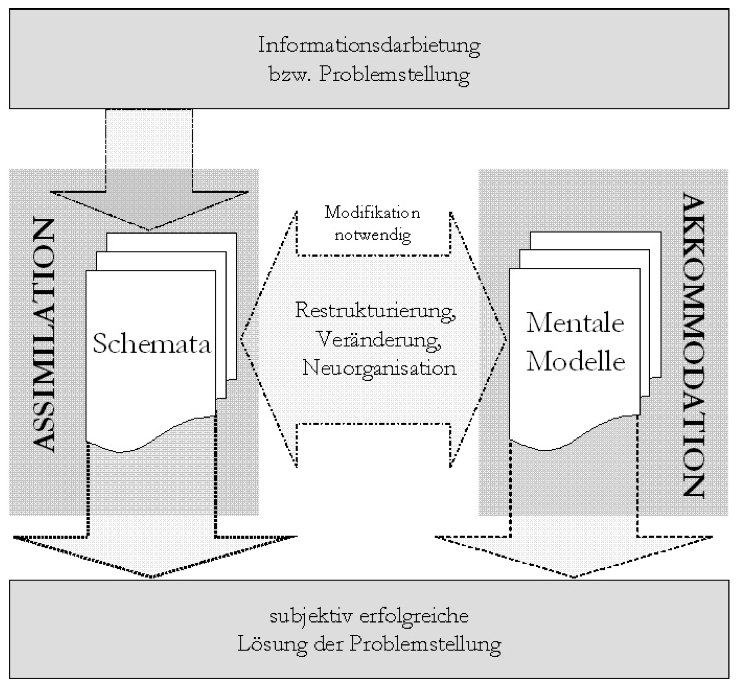
\includegraphics[height=3in]{img/MentaleModelle/iffenthaler_assimilation_akkommodation.png}
	\caption[Schemata und mentale Modelle]{Schemata und mentale Modelle (entnommen aus \citet[][S. 10]{Ifenthaler06})}
	\label{fig:img_MentaleModelle_iffenthaler_assimilation_akkommodation}
\end{figure}

Solange \wichtig eine wahrgenommene Situation auf existierende Schemata abgebildet werden kann und daraus unmittelbar Handlungen abgeleitet werden können, spricht man von „Assimilation“ der wahrgenommene Information. „Assimilation“ festigt bestehende Schemata, gestaltet diese ggf. in Details exakter aus oder um, stellt die grundlegenden Annahmen, die dem Schema zugrunde liegen, aber nicht in Frage. Kann die wahrgenommene Information nicht auf existierende Schemata abgebildet werden, kommt es zur „Akkommodation“, also der (ad-hoc) Bildung eines mentalen Modells und darauf aufbauend zur \emph{„Restrukturierung, Veränderung und Neuorganisation“} \citep{Ifenthaler06} der betreffenden Schemata. Schemata und mentale Modelle können damit auch als jene Strukturen interpretiert werden, die beim „Single-“ bzw. „Double-Loop-Learning“ nach \citet{Argyris78} zum Einsatz kommen. Im Kontext von „Articulation Work“ sind mentale Modelle in jenen Situation von Interesse, die als so „problematisch“ wahrgenommen werden, dass keine Fortführung der operativen Arbeit mehr möglich ist (auf individueller Ebene also evtl. existierende „Schemata“ nicht mehr zum Einsatz gebracht werden können). In diesen Situationen muss „explizite Articulation Work“ durchgeführt werden, um auf Basis eines mentalen Modells dieses selbst zu verändern, auszugestalten und soweit mit der Umwelt abzustimmen, das eine Wiederaufnahme der operativen Arbeit (bzw. die Bildung von adäquaten Schemata) möglich wird. Um auf die Durchführung von „expliziter Articulation Work“ unter Bezugnahme auf die mentalen Modelle der Individuen näher eingehen zu können, werden im nächsten Abschnitt die Bildung und Veränderung mentaler Modelle näher betrachtet.

\section{Bildung und Veränderung mentaler Modelle} % (fold)
\label{sec:bildung_mentaler_modelle}

Nach \citep{Seel91} umfasst die Bildung mentaler Modelle zwei Komponenten: Eine \emph{deklarative Komponente}, in der bereichs- bzw. domänen-spezifisches Wissen in der Form von hier nicht näher spezifizierten, strukturierten Wissensbasen abgelegt wird und eine \emph{operative Komponente}, in der auf Grundlage dieser Wissensbasen Schlüsse gezogen und neues Wissen abgeleitet wird, die über das ursprüngliche domänenspezifische Wissen hinausgeht. 

Das in den Wissensbasen repräsentierte Wissen kann auf Alltagserfahrung begründet sein oder durch Vermittlung oder Instruktion begründet werden. Im ersteren Fall ist das Wissen dann als konkret und handlungsbezogen angesehen werden, im zweiten Fall ist das Wissen eher auf abstrakter, formaler Ebene anzusiedeln. Analog dazu kann auch in der operativen Komponente die Schlussfolgerung induktiv auf Basis eines „intuitionsbegründeten“ Regelsystems gezogen werden oder durch Deduktion mittels einem formal begründbaren Regelsystem gebildet werden. 

Die Modifikation und Erweiterung der eigenen Wissensbasen und die (Weiter-)Entwicklung der kognitiven Fähigkeiten, die für die Ableitung von Schlussfolgerungen notwendig sind, bezeichnet \citet{Seel91} als „Lernen“. Lernen ist \emph{"mit der Verarbeitung individueller Erfahrungen mit sowie vermittelter Information über die Welt, ihre Struktur und Evidenz verbunden und kann als ein Prozess permanenter konzeptueller Veränderungen verstanden werden."} \citep[][S. 23]{Seel91}. Lernen setzt damit die Fähigkeit und Bereitschaft voraus, \emph{"vermittelte Weltauffassungen zu verstehen, zu akzeptieren und sodann den eigenen gedanklichen Konstruktionen zugrunde zu legen"} \citep[][S. 23]{Seel91}. Im Wesentlichen entspricht dies einer Verallgemeinerung jener Vorgänge die im Rahmen von nicht rein koordinierender sondern abstimmender und vor allem planender „Articulation Work“ durchgeführt werden.

In diesem Zusammenhang sind verschiedene Arten von mentalen Modellen zu unterscheiden. \citet{Seel91} differenziert zwischen „Novizenmodellen“ und „Expertenmodellen“. Ein „Novizenmodell“ ist ein Alltagsmodell, dass ad-hoc in einer Problemsituation gebildet wird und ist im dem Individuum, das es gebildet hat, in der aktuellen Situation plausibel (auch wenn es objektiv falsch ist). Es ist ausreichend, um adäquate Reaktionen auf die gegebene Situation abzuleiten, ohne das notwendigerweise eine Begründung der Handlungen möglich ist oder diese nicht mit dem tatsächlichen Grund der Problembewältigung übereinstimmen\footnote{\emph{„[\ldots] most people’s understanding of the devices they interact with is surprisingly meager, imprecisely specified, and full of inconsistencies, gaps and idiosyncratic quirks.“}\citep[][S. 8]{Norman83a}}. Je öfter die Anwendung eines „Novizenmodells“ zum Erfolg führt, umso stabiler wird es zur Grundlage des Handelns des Individuums in der jeweiligen Situation. „Expertenmodelle“ (oder „wissenschaftliche Modelle“) sind hingegen inhaltlich vollständiger und bilden die Ursache-Wirkungs-Zusammenhänge der beobachtbaren Realität ab (sind also „objektiv korrekt“). Sie sind im allgemeinen differenzierter und bedienen sich einer adäquateren mentalen Codierung als „Novizensysteme“ (die sich i.A. existierender mentale Codierungen bedienen). Auch die Kompetenz des Individuums im Umgang mit dem mentalen Modell ist in diesem Fall höher. Der Übergang von einem „Novizenmodell“ zu einem „Expertenmodell“ erfolgt dabei durch „Lernen“ im oben genannten Sinn. \citep{Ifenthaler06}

„Expertenmodelle“ müssen aber nicht immer den erwünschten Endzustand eines Lernprozesses darstellen. Durch die gesteigerte Komplexität des Modells wird dessen ad-hoc-Anwendung schwieriger, die Nützlichkeit des Modells ist deshalb eingeschränkt \citep[vgl. ][S. 20]{Ifenthaler06}. Hier zeigt sich wiederum eine Analogie mit dem Bereich „Articulation Work“, wo es -- wie im letzten Kapitel beschrieben -- ebenfalls nicht als erforderlich angesehen wird, dass jedes beteiligte Individuum eine detaillierte Gesamtsicht auf den Arbeitsablauf hat sondern es ausreichend ist, die jeweils relevanten Schnittstellen zu abzustimmen und einen groben Überblick über den Gesamtzusammenhang zu haben. 

\citet{Ifenthaler06} erweitert deshalb die binäre Klassifikation durch „Erklärungsmodelle“, die er konzeptionell zwischen „Novizen-“ und „Expertenmodellen“ ansiedelt. Ein „Erklärungsmodell“ \emph{„beinhaltet alle notwendigen Informationen, um ein Problem bezüglich des Sachverhaltes und der Anforderungssituation richtig zu lösen. Einem Erklärungsmodell wird dabei ein hoher Grad an Nützlichkeit beigemessen, was in Bezug auf die kognitive Leistung zu einer ergonomischen Problemlösung führt. Je nach Komplexität des Sachverhaltes und der damit verbundenen Anforderungssituation kann ein Erklärungsmodell einem Novizenmodell oder einem Expertenmodell sehr ähnlich sein“} \citet[][S. 21]{Ifenthaler06}. „Erklärungsmodelle“ sind also je nach Art der zugrunde liegenden Problemstellung unterschiedlich aufgebaut. Ziel eines „Erklärungsmodells“ ist es immer, bestmöglich zur Problemlösung beizutragen, diese also für das Individuum im Kontext der jeweiligen Problemstellung möglichst einfach zu gestalten. Ein „Erklärungsmodell“ gewinnt dabei durch „Lernen“ an Reifegrad, es nähert sich einem „Expertenmodell“ immer weiter an.

Im \wichtig Kontext von „Articulation Work“ ist der Begriff des „Erklärungsmodells“ ein hilfreiches Konstrukt. Je nach Reifegrad des betreffenden mentalen Modells wird eine bestimmte Arbeitssituation als mehr oder weniger komplex wahrgenommen. Je komplexer eine Arbeitssituation wahrgenommen wird, desto größer ist der Bedarf nach expliziter „Articulation Work“, also der expliziten Beschäftigung mit dem Arbeitsprozess, dessen Reflexion und der Abstimmung der eigenen Wahrnehmung mit anderen beteiligten Individuen. Diese Beschäftigung mit dem Arbeitsprozess, also jene Tätigkeiten, die im Rahmen der „Articulation Work“ durchgeführt werden, entsprechen -- wie oben bereits beschrieben -- dem hier beschriebenen „Lernen“, wobei in kooperativen Arbeitssituation die Quellen „vermittelter Information“ vorrangig die anderen beteiligten Individuen oder organisationale Artefakte sind, die den Arbeitsablauf beschreiben. 

Die Veränderung mentaler Modelle weist zwei grundlegende Schwierigkeiten auf. Bei bereits als nicht adäquat erkannten mentalen Modellen (wie sie bei „Articulation Work“, die in „non-routine work“ bzw. „problematic work“ ausgeführt wird, auftreten), besteht grundsätzlich die Bereitschaft zur Veränderung (im Sinne einer „Akkommodation“ des mentalen Modells an die als verändert wahrgenommene Umweltbedingungen), die Herausforderung besteht aber darin, die notwendigen Informationen vermittelt zu bekommen also an diese zu gelangen und diese adäquat dargeboten zu bekommen. Eine weitere Schwierigkeit ergibt sich in Situationen, in denen nicht alle involvierten Individuen die Situation als „problematisch“ wahrnehmen und deshalb keine grundlegende Bereitschaft zeigen, ihre der Arbeit zugrunde liegenden Annahmen (also ihre mentalen Modelle) zu verändern (\citep{Ifenthaler06} spricht von „hoher Veränderungsresistenz“). Dies tritt vor allem im Situationen auf, in denen „Articulation Work“ nicht aus einer allgemein wahrgenommen Problemsituation heraus durchgeführt wird, sondern entweder mit rein planendem Charakter angestoßen wird oder nur für einzelnen beteiligte Individuen so stark „problematisch“ ist, dass eine explizite Beschäftigung mehrerer oder aller am Arbeitsablauf beteiligten notwendig ist. 

Grundsätzlich müssen also aus der Theorie der mentalen Modelle heraus begründet zu erfolgreicher „expliziter Articulation Work“ drei Rahmenbedingungen gegeben sein:
\begin{enumerate}
	\item Die Beteiligten müssen bereit sein, ihre mentalen Modelle abzustimmen und das individuelle Verständnis der Schnittstellen abzugleichen.
	\item Die von den beteiligten Individuen benötigte Information über den Arbeitsablauf muss von den anderen Beteiligten zur Verfügung gestellt werden können oder in der Form organisationaler Artefakte vorliegen.
	\item Die benötigte Information muss in adäquater Form dargeboten werden, um  die individuellen mentalen Modellen mit diesen in Einklang zu bringen.
\end{enumerate}

Anforderung 1 ist eine Frage des sozialen Verhaltens der beteiligten Personen bzw. der Organisationskultur und kann ggf. durch organisationale Maßnahmen (z.B. durch die Förderung von „Communities of Practice“ \citep{Wenger99}) unterstützt werden. Anforderung 2 kann trivial zu erfüllen sein, wenn der Kontext des Arbeitsablaufs (d.h. das Umfeld, in dem die Arbeit durchgeführt wird, u.a. inkl. aller beteiligten Individuen) bekannt ist. In komplexen, neuartigen oder unbekannten Arbeitssituationen muss auch die Erfüllung dieser Anforderung unterstützt werden. Ansatzpunkte dafür liefert im Bereich von „Articulation Work“ etwa \citep{Grinter96} oder \citep{Fuchs01}, umfassend mit dieser Thematik beschäftigt sich der Forschungsbereich der „Organisational Memories“ (zur technischen Unterstützung siehe etwa \citep{Abecker98} oder \citep{Diefenbruch02}\footnote{eine detaillierte Darstellung des Forschungsgebiets ist in \citep{Maier08} zu finden}).

Anforderung 3 wird in der Forschung zum Thema „Articulation Work“ von \citet{Sarini02} im Kontext des „alignment of meanings“ angesprochen, bei dem eine automationsgestützte Abbildung unterschiedlicher Domänenvokabulare die grundsätzliche Verständigung bzw. die Vermeidung von Missverständnissen vermeiden soll. Diese Maßnahme ermöglicht allerdings erst die Abstimmung mentaler Modelle, unterstützt diese aber noch nicht unmittelbar. Im Sinne der adäquaten Form der Darbietung argumentieren auch \citep{Divitini00}, \citep{Jorgensen04} und vor allem 
\citep{Herrmann02} mit der Forderung von flexiblen bzw. an die Bedürfnisse der Benutzer anpassbaren Modellierungsprachen bei der Verwendung von externalisierten Modellen als Unterstützung der Durchführung von „Articulation Work“. 

Hinsichtlich \wichtig Anforderung 3 argumentiert \citet{Seel91} im Bereich der mentalen Modelle ebenfalls für die Nützlichkeit externalisierter Repräsentationen zur Verbesserung von mentalen Modellen. Er vertritt die Auffassung, dass „die Externalisierung die Konstruktion eines mentalen Modells 'vervollkommnet'“, was er darauf zurückführt, dass „erst aus der Zielsetzung heraus, sich einem anderen mitzuteilen, die Präzision einer gedanklichen Konstruktion resultiert, die für die Erklärung einer Weltergebenheit erforderlich ist“ \citep[][S. 155]{Seel91}. Die Bildung von Externalisierungen mentaler Modelle verbessert also einerseits das individuelle mentale Modell, indem sie Lücken und Inkonsistenzen bewusst macht, und ermöglicht andererseits die Kommunikation mit anderen Individuen und ist damit die Grundlage der Vermittlung von Information und damit des „Lernens“ und „Articulation Work“ im hier beschriebenen Sinn. \citet{Seel91} lässt jedoch offen, in welcher Form die Repräsentation erfolgt, um die Vermittelbarkeit bestmöglich sicherzustellen\footnote{\emph{„Internalisierung von Erkenntnismitteln setzen Zeichensysteme (auditiver, visueller oder anderer Natur) für die Verschlüsselung der semantischen Gebilde voraus“}\citep[][S. 155]{Seel91}}. \citet{Ifenthaler06}, \citet{Hanke06} und \citep{Pirnay-Dummer06} weisen an dieser Stelle jedoch auf qualitative Unterschiede der Eignung unterschiedlicher externer Repräsentationsformen mentaler Modelle zur Externalisierung und Vermittlung derselben hin. Auf diese unterschiedlichen Formen und deren Eignung wird im nächsten Abschnitt eingegangen. 

Grundsätzlich konnte jedoch hier gezeigt werden, dass „Articulation Work“ in ihren komplexen Ausprägungen die mentalen Modelle der beteiligten Individuen verändert bzw. auf diesen aufbaut. In weiterer Folge wurde deutlich, dass zur expliziten Durchführung von „Articulation Work“ auch aus der Theorie der mentalen Modelle heraus die Verwendung von externalisierten Modellen (wie bereits von \citep{Divitini00}, \citep{Herrmann02} und \citep{Jorgensen04} ohne den Hintergrund der mentalen Modelle vorgeschlagen) sinnvoll ist.
% section bildung_mentaler_modelle (end)

\section{Externalisierung mentaler Modelle} % (fold)
\label{sec:externalisierung_mentaler_modelle}

Die Externalisierung von „mentalen Modellen“ ist immer ein zweistufiger Prozess (siehe Abbildung \ref{fig:img_MentaleModelle_iffenthaler_externalisierung}), in dem jeweils eine Transformation des Kodierungssystems stattfindet. Die wahrgenommene Realität (das „Weltwissen“) wird (ad-hoc) in ein mentales Modell abgebildet werden. Soll dieses externalisiert werden, ist dazu ein weiterer Übersetzungs- bzw. Abbildungsschritt notwendig. Gleichzeitig führt jede Modellbildung nach \citet{Stachowiak73} neben der „Abbildung“ auch zur „Verkürzung“, d.h. dass das Modell nicht die gesamte Information des Originals enthält, sondern nur jene Aspekte, die dem Ersteller relevant erscheinen. In diesem Sinne können sie nur in einem bestimmten (zeitlichen, personellen und operationalen) Kontext für das Original stehen („pragmatisches Merkmal“ -- jedes Modells ist für einen bestimmten Zweck konstruiert).

\begin{figure}[htbp]
	\centering
		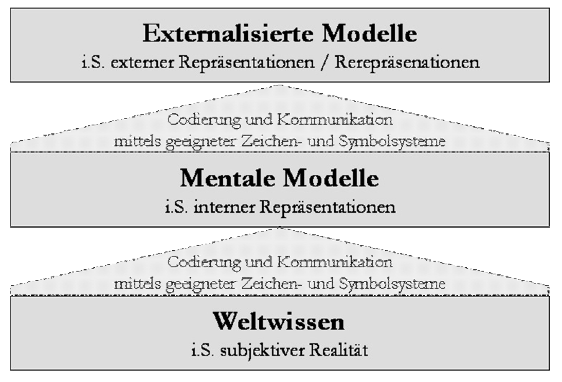
\includegraphics[width=5cm]{img/MentaleModelle/iffenthaler_externalisierung.png}
	\caption[Externalisierung mentaler Modelle]{Externalisierung mentaler Modelle (entnommen aus \citep{Ifenthaler06})}
	\label{fig:img_MentaleModelle_iffenthaler_externalisierung}
\end{figure}

Herausfordernd ist im Kontext von „Articulation Work“ das Abbildungsmerkmal, also die notwendige Übersetzungsleistung bei der Externalisierung eines mentalen Modells. Externalisierung umfasst nach \citet{Hanke06} immer die „Repräsentation“ als auch die „Kommunikation“ eines mentalen Modells. Die Relevanz dieser beiden Aspekte verschiebt sich je nach Kontext bzw. Zielsetzung der Externalisierung. Dient diese eher der individuellen Verständnisbildung, steht die „Repräsentation“ im Vordergrund (diesen Zweck erfüllt nach \citep{Seel91} auch bereits das mentale Modell selbst, die Externalisierung hat schärfenden Charakter). Die externalisierte Repräsentation soll nach \citet[][S. 187]{Seel91} in Bezug auf das repräsentierte mentale Modell
\begin{itemize}
	\item vollständig 
	\item konzise
	\item kohärent und konkret
	\item bedeutungshaltig und korrekt
\end{itemize}
sein. Das Kodierungssystem muss hier also so gewählt werden, dass eine möglichst unmittelbare Abbildung der mentalen Modelle auf die externalisierte Repräsentation (und vice versa) möglich ist. 

In Situationen, in denen mentale Modelle zusätzlich auch anderen Individuen vermittelt werden sollen, steht „Kommunikation“ im Vordergrund. Die „Kommunizierbarkeit“ eines mentalen Modells hat Auswirkungen auf die wählbaren Kodierungssysteme zur Externalisierung. Das gewählte Kodierungssystem muss allen beteiligten Individuen verständlich sein, während dieses Kriterium bei der individuellen Verständnisbildung irrelevant ist \citep{Hanke06}. Im Rahmen von „Articulation Work“ steht im Allgemeinen die „Kommunikation“ bei der Externalisierung im Vordergrund, wobei diese ohne eine adäquate „Repräsentation“ nicht möglich ist. Ziel muss es also sein, Kodierungssysteme zur Verfügung zu stellen, die 
\begin{itemize}
	\item allen beteiligten Individuen verständlich sind, und
	\item eine möglichst unmittelbare Abbildbarkeit der mentalen Modelle auf die externalisierte Repräsentation ermöglicht.
\end{itemize}

Kodierungssysteme können \emph{„auditiver, visueller oder anderer Natur“}\citep[][S. 155]{Seel91} sein. Das gebräuchlichste Kodierungssystem ist die natürliche Sprache. Diese ist im Sinne der ersten Anforderung oft eine gute Wahl, bietet aber aufgrund ihrer Generizität nur wenig Möglichkeiten, sowohl den Repräsentations- als auch den Kommunikationsprozess bei der Externalisierung explizit zu unterstützen. \citet{Ifenthaler06} stellt mehrere Methoden vor, die sich spezifisch zum Zwecke der Externalisierung mentaler Modelle eignen und zu qualitativ höherwertigen Externalisierungsergebnisse führen sollen. Dies sind im Einzelnen:
\begin{itemize}
	\item Methode des lauten Denkens
	\item Strukturlegetechniken
	\item Concept Mapping
\end{itemize}

Diese Ansätze werden in der Folge detaillierter betrachtet. Dabei kommt folgender Raster zum Einsatz:
\begin{description}
	\item[Konzept] beschreibt die grundlegenden Konzepte des Ansatzes und die darauf aufbauende Zielvorstellung
	\item[Vorgehen] beschreibt, wie die Zielerreichung methodisch sichergestellt werden soll. 
	\item[Unterstützung] beschreibt, welche (technischen) Unterstützungsmaßnahmen vorgeschlagen werden.
\end{description}

\subsection{Methode des lauten Denkens} % (fold)
\label{sub:methode_des_lauten_denkens}

% subsection methode_des_lauten_denkens (end)

\subsection{Strukturlegetechniken} % (fold)
\label{sub:strukturlegetechniken}

Variante: Test für Kausalmodelle (vgl. \citep[][S. 32]{Ifenthaler06})
% subsection strukturlegetechniken (end)

\subsection{Concept Mapping} % (fold)
\label{sub:concept_mapping}

% subsection concept_mapping (end)

% section externalisierung_mentaler_modelle (end)

% chapter mentale_modelle (end)

% \chapter{Mentale Modelle}
% \label{cha:mentale_modelle}
% 
% In diesem Kapitel wird das Konzept der mentalen Modelle eingeführt, das in dieser Arbeit als Erklärungsansatz für jene Aspekte von "Articulation Work" verwendet wird, die die nicht sichtbaren, kognitiven Beiträge eines beteiligten Individuums betreffen. Nach einer Einführung in die Begriffswelt der mentalen Modelle wird die Argumentation aus dem letzten Kapitel nochmals aufgegriffen und die mögliche Rolle mentaler Modelle für "Articulation Work" erörtert. In der Folge werden Methoden eingeführt mit denen mentale Modelle externalisiert und kommuniziert werden können. Basierend auf diesen Beschreibungen wird im letzten Teil des Kapitels untersucht, welche Herausforderungen sich bei der Anwendung dieser Methoden im Kontext von "Articulation Work" ergeben können.
% 
% \section{Begriffsbestimmung}e
% \label{sec:mentalemodelle_begriffsbestimmung}
% 
% Der Begriff der Mentalen Modelle wurde von \citet{Johnson-Laird81} geprägt. Ein mentales Modell ist nach 
% 
% \subsection{Mentale Modelle nach Johnson-Laird} % (fold)
% \label{sub:mentale_modelle_nach_johnson_laird}
% 
% % subsection mentale_modelle_nach_johnson_laird (end)
% 
% \subsection{Mentale Modelle nach Norman} % (fold)
% \label{sub:mentale_modelle_nach_norman}
% 
% \citet{Norman83a} formuliert ein Verständnis von mentalen Modellen aus Interaktionssicht. Sein Kontext ist die Untersuchung von Mensch-Maschine-Interaktion und den dort auftretenden Interaktionsabläufen. Mentale Modelle sind in diesem Verständnis individuelle Konstrukte, die von Menschen bei der Interaktion mit der Umwelt, mit anderen Menschen oder mit Technologie gebildet werden, um das Verhalten der Gegenseite erklären und vorhersagen zu können\footnote{\emph{„In interaction with the environment, with others, an with the artifacts of technology, people form internal, mental models of themselves and of the things with which they are interacting. These models provide predictive and explanatory power for understanding the interaction“} \citep{Norman83a}}. Um den Begriff abzugrenzen, führt \citeauthor{Norman83a} ein aus vier Elementen bestehendes Begriffssystem ein, das den Diskussionsbereich abgrenzt und definiert:
% \begin{description}
% 	\item[target system] Das Zielsystem ist jenes System, das von einer Person benutzt wird oder dessen Benutzung von dieser Person erlernt wird.
% 	\item[conceptual model of target system] Ein konzeptionelles Modell ist ein Modell, dass das Zielsystem vollständig, konsistent und exakt beschreibt. Konzeptionelle Modelle werden von Entwicklern, Designern, Wissenschaftern oder Lehrern (im Allgemeinen: Experten in der Domäne des Zielsystems) definiert.
% 	\item[mental model of target system] Mentale Modelle werden von Personen bei der Interaktion mit dem Zielsystem entwickelt, um dessen Verhalten zu erklären. Diese Modelle müssen nicht vollständig und exakt sein, müssen aber für die jeweilige Person funktional sein, d.h. für deren Zwecke ausreichendes Erklärungspotential besitzen. Mentale Modelle haben evolutionären Charakter und entwickeln sich während der Interaktion mit dem System weiter. Die Inhalte eines mentalen Modells werden durch das Vorwissen und die Erfahrung der jeweiligen Person beeinflusst.
% 	\item[scientist's conceptualization of mental model] Die Konzeptualisierung eines mentalen Modells ist der Versuch ein mentales Modell mit wissenschaftlichen Mitteln zu erheben und abzubilden. Sie soll die Inhalte des mentalen Modells möglichst vollständig und genau abbilden. Die Konzeptualisierung ist also ein Modell eines Modells.
% \end{description}
% 
% Im Weiteren nennt \citeauthor{Norman83a} sechs generelle Eigenschaften von mentalen Modellen, die er aus eine Vielzahl von Beobachtungen in unterschiedlichen Kontexten ableitet:
% \begin{enumerate}
% 	\item Mentale Modelle sind unvollständig
% 	\item Mentale Modelle können von ihren Trägern nur sehr einschränkt wiedergegeben werden.
% 	\item Mentale Modell sind instabil und werden vor allem in Bereich ungenau, die Teile des Zielsystems abbilden die lange nicht benötigt wurden.
% 	\item Mentale Modelle sind nicht klar voneinander abgrenzbar -- ähnliche Gegenstände oder Situationen werden oft hinsichtlich der angewandten Interaktionsmuster verwechselt.
% 	\item Mentale Modelle sind unwissenschaftlich -- auch mentale Modelle, die inhaltlich (technisch) überflüssiges Verhalten verursachen, werden beibehalten, wenn der Aufwand der physischen Ausführung gering ist.
% 	\item Mentale Modelle sind simpel -- auch wenn eine effizientere Interaktion möglich wäre, wenn mehr Aufwand in die Planung investiert würde bzw. ein komplexeres mentales Modell zum Einsatz käme, präferieren Benutzer einfache Modelle, deren Anwendung höheren „physischen Aufwand“ mit sich bringen.
% \end{enumerate}
% 
% % subsection mentale_modelle_nach_norman (end)
% 
% \subsection{Mentale Modelle nach Senge} % (fold)
% \label{sub:mentale_modelle_nach_senge}
% 
% % subsection mentale_modelle_nach_senge (end)
% 
% \section{Veränderung mentaler Modelle}
% \label{sub:veränderung_mentaler_modelle}
% Assimilation vs. Akkommodation
% 
% \section{Mentale Modelle und Articulation Work}
% \label{sec:mentale_modelle_und_articulation_work}
% 
% Argumentation mit Wissensspirale (Nonaka \& Takeuchi)
